\chapter{Results and Discussion}
\label{chap:results}
\noindent \rule{6.6in}{0.01in}
\newpage

\section{Overall Model Comparison}

Table~\ref{tab:overall-comparison} and Figure~\ref{fig:model-comparison} summarise how the five models -- the four base classifiers and the stacked ensemble -- perform on the held-out test set of 1{,}635 events. Every model lands in the 89--93\% range on raw accuracy, which at first glance looks like a fairly narrow, unremarkable spread. Macro-F1, which averages performance across all four severity classes \emph{without} weighting by how common each class is, tells a much less flattering story: it ranges from 0.5843 (the MLP) up to 0.6949 (LightGBM), a gap far too large to be explained by the near-identical accuracy figures above it.

\begin{table}[!h]
\centering
\caption{Overall performance on the held-out test set (n = 1{,}635).}
\label{tab:overall-comparison}
\begin{tabular}{lccc}
\toprule
Model & Accuracy & Macro-F1 & Weighted-F1 \\
\midrule
LightGBM         & 0.9223 & \textbf{0.6949} & 0.9148 \\
XGBoost          & 0.9168 & 0.6906 & 0.9114 \\
MLP-NN           & 0.9242 & 0.5843 & 0.8992 \\
TabNet           & \textbf{0.9254} & 0.6027 & 0.9020 \\
Stacked Ensemble & 0.8948 & 0.6639 & 0.8968 \\
\bottomrule
\end{tabular}
\end{table}

\begin{figure}[!h]
\centering
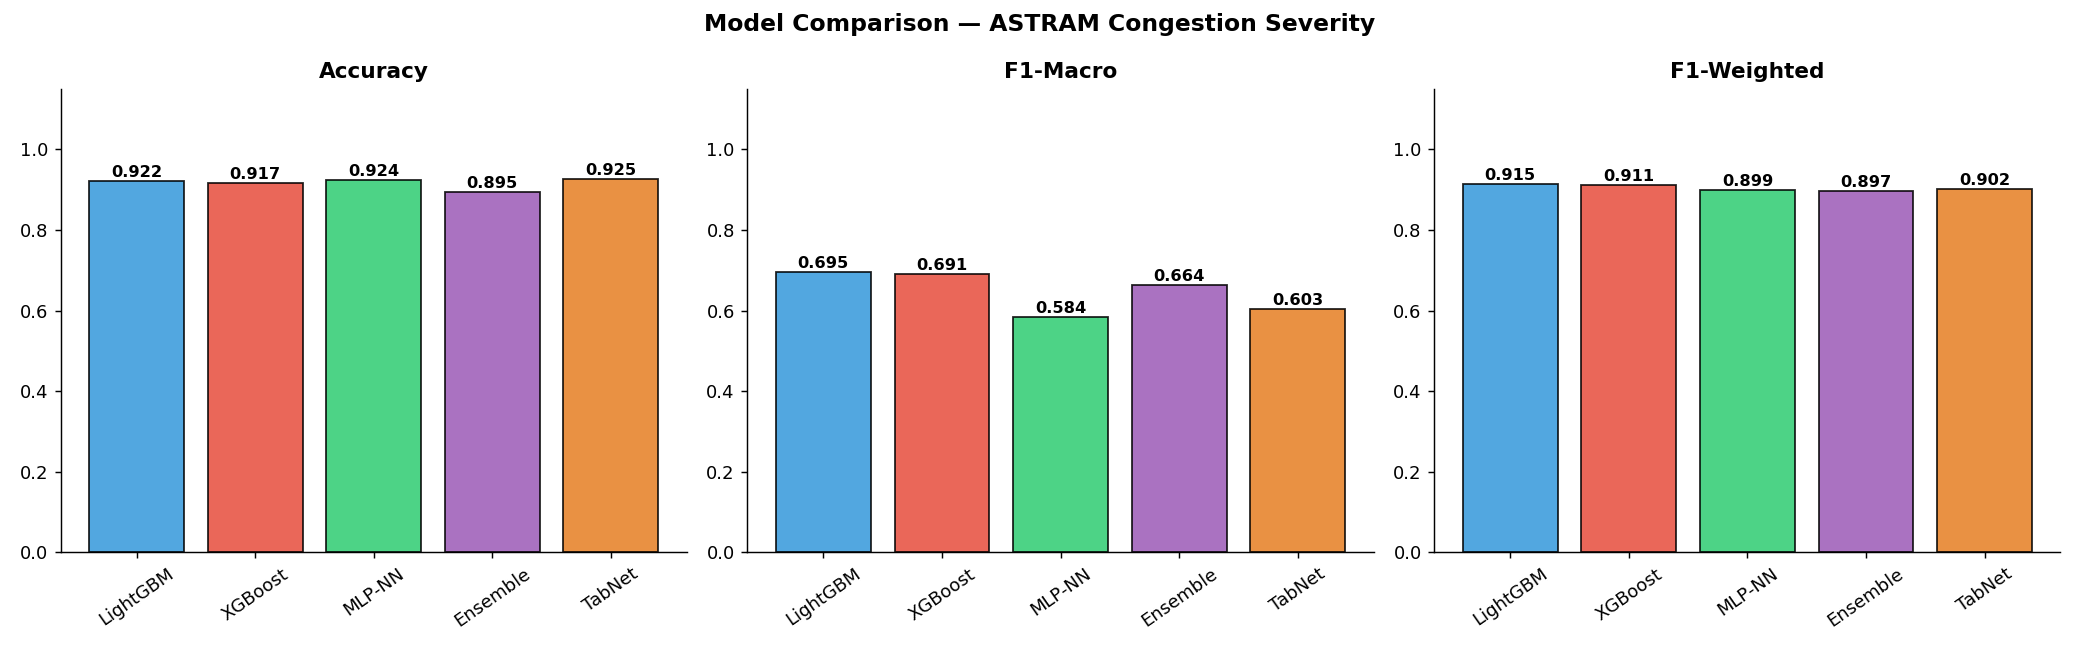
\includegraphics[width=0.95\textwidth]{chapters/7/figs/model_comparison.png}
\caption{Accuracy, macro-F1, and weighted-F1 across all five models.}
\label{fig:model-comparison}
\end{figure}

It is worth flagging the reversal directly: TabNet posts the single highest accuracy of the five models (0.9254), yet it is \emph{not} the best model on macro-F1 -- that title goes to LightGBM, whose accuracy (0.9223) is marginally lower. This is the first sign, examined in depth over the next two sections, that ranking these models by accuracy alone would point a deployment decision in the wrong direction.

\section{Per-Class Performance and the Class-Imbalance Effect}

Table~\ref{tab:critical-class} and Figure~\ref{fig:critical-recall} zoom in on the Critical class specifically, since a missed Critical event is the single costliest mistake this system can make.

\begin{table}[!h]
\centering
\caption{Critical-class precision, recall, and F1-score by model (support = 59).}
\label{tab:critical-class}
\begin{tabular}{lccc}
\toprule
Model & Precision & Recall & F1-score \\
\midrule
LightGBM         & 0.54 & 0.32 & \textbf{0.40} \\
XGBoost          & 0.46 & 0.36 & \textbf{0.40} \\
MLP-NN           & 1.00 & 0.03 & 0.07 \\
TabNet           & 0.75 & 0.10 & 0.18 \\
Stacked Ensemble & 0.28 & 0.34 & 0.31 \\
\bottomrule
\end{tabular}
\end{table}

\begin{figure}[!h]
\centering
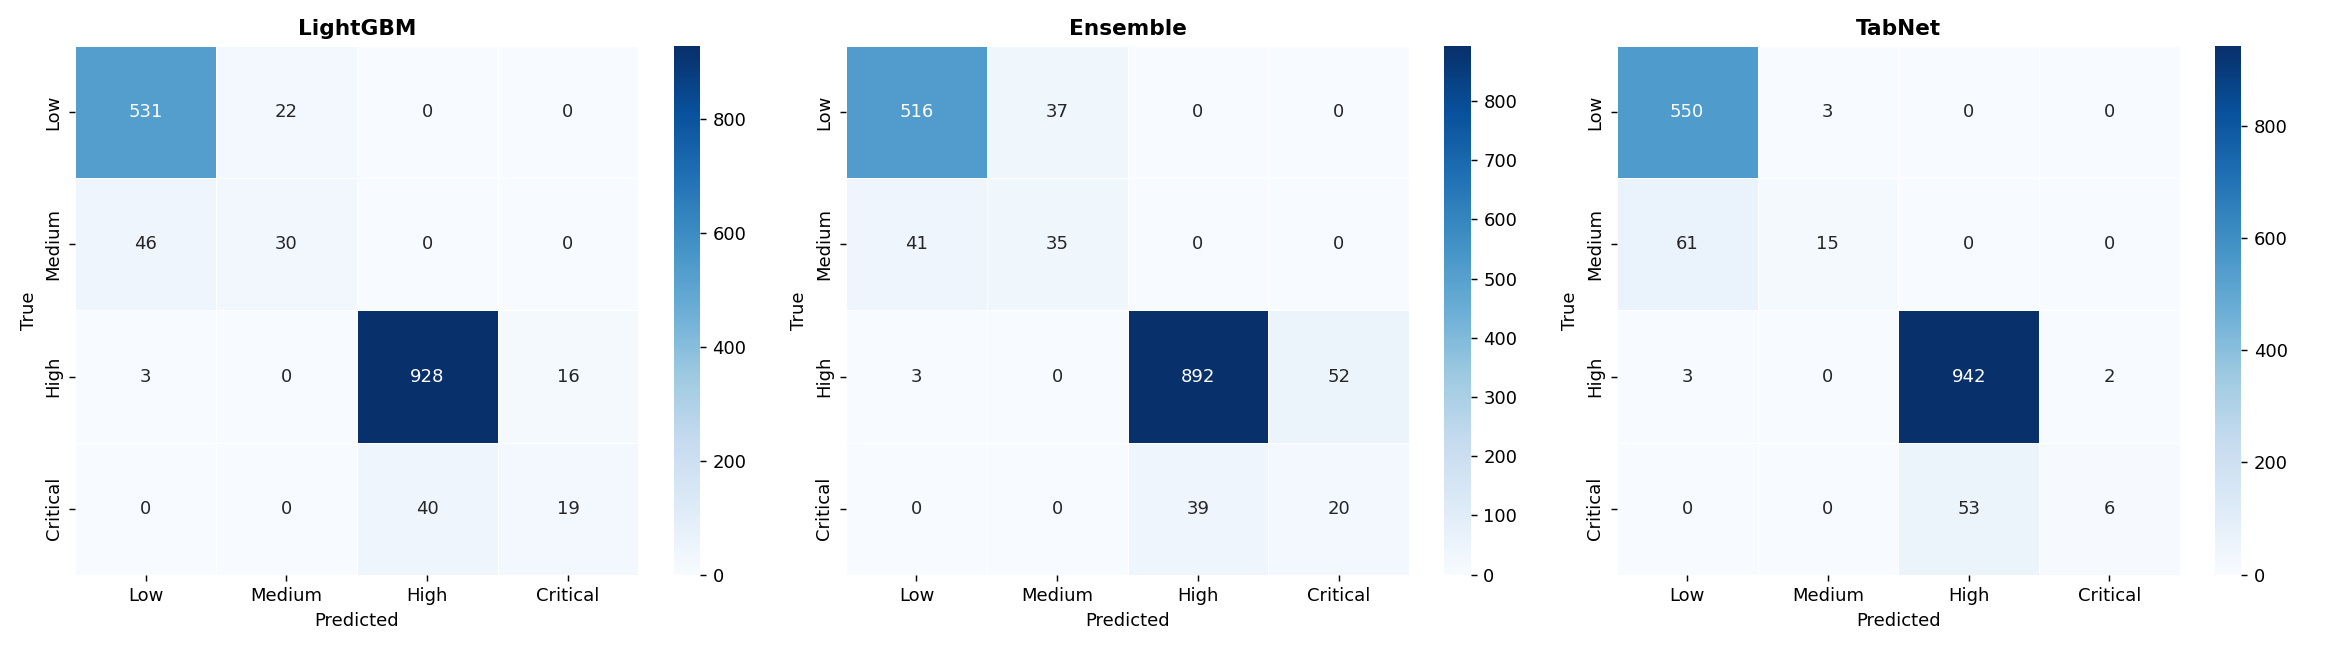
\includegraphics[width=0.75\textwidth]{chapters/7/figs/confusion_matrices.png}
\caption{Confusion matrices for LightGBM, the stacked ensemble, and TabNet on the test set.}
\label{fig:critical-recall}
\end{figure}

The MLP row in Table~\ref{tab:critical-class} is the clearest illustration of the failure mode this thesis is built around: a precision of 1.00 alongside a recall of only 0.03 means that whenever the MLP does predict Critical, it happens to be right every time, but it only makes that prediction for 3\% of the 59 truly Critical events in the test set -- it silently lets the other 97\% through mislabelled as something less urgent. TabNet shows a softer version of the same pattern (75\% precision, 10\% recall). LightGBM and XGBoost, the two models trained with explicit class-balanced sample weighting, behave quite differently: their Critical recall sits at 0.32 and 0.36 respectively, and they end up as the two best-performing models on Critical-class F1 (0.40 each) even though neither of them had the best overall accuracy in Table~\ref{tab:overall-comparison}.

A milder version of the same pattern shows up for the Medium class (Table~\ref{tab:medium-class}): LightGBM and the stacked ensemble share the best Medium-class F1 (0.47), clearly ahead of the MLP (0.36) and TabNet (0.32).

\begin{table}[!h]
\centering
\caption{Medium-class precision, recall, and F1-score by model (support = 76).}
\label{tab:medium-class}
\begin{tabular}{lccc}
\toprule
Model & Precision & Recall & F1-score \\
\midrule
LightGBM         & 0.58 & 0.39 & \textbf{0.47} \\
XGBoost          & 0.56 & 0.39 & 0.46 \\
MLP-NN           & 0.75 & 0.24 & 0.36 \\
TabNet           & 0.83 & 0.20 & 0.32 \\
Stacked Ensemble & 0.49 & \textbf{0.46} & \textbf{0.47} \\
\bottomrule
\end{tabular}
\end{table}

For contrast, all five models handle the two majority classes comfortably -- Low-class F1 sits at 0.93--0.94 and High-class F1 at 0.95--0.97 across the board, regardless of which model is used. The entire spread in Table~\ref{tab:overall-comparison}'s macro-F1 column, in other words, is coming almost entirely from how each model treats the two rarer classes, which is exactly what the accuracy figures alone hide.

\section{Why the Stacked Ensemble Did Not Improve Accuracy}

One result that runs against the usual expectation of stacking is that the ensemble does \emph{not} come out on top of either accuracy or macro-F1 -- it actually posts the lowest raw accuracy of all five models (0.8948), even though its macro-F1 (0.6639) is comfortably ahead of both neural models. Two things plausibly explain this. First, the base models trained inside the five-fold out-of-fold loop were deliberately lighter than their final, fully-tuned counterparts reported in Table~\ref{tab:overall-comparison} -- the in-fold MLP, for instance, uses only two hidden layers (128, 64) rather than the four-layer (256, 128, 64, 32) architecture used for the standalone MLP result -- which likely makes the out-of-fold probability estimates the meta-learner trains on noisier than the probabilities it sees at test time. Second, with only 297 Critical and 379 Medium examples in the whole dataset, five-fold cross-validation leaves each fold with well under 100 examples of either class, which limits how reliably the meta-learner can learn class-specific combination weights for exactly the classes that matter most. Even so, the ensemble still ties for the best Medium-class F1 and posts the second-best Critical recall of all five models, which suggests it is doing what it was built to do -- spreading detection more evenly across classes -- just at some cost to overall accuracy in this particular run.

\section{Why Accuracy Alone Is an Unreliable Metric Here}

Put the two previous sections together and the practical risk becomes concrete rather than abstract: with 91.7\% of the test set being either Low or High severity, a model that leans hard into predicting those two classes can clear 92\% accuracy while missing almost every Critical event it was meant to catch. That is not a hypothetical failure mode -- it is exactly what the MLP does in this experiment, reporting 92.4\% accuracy alongside 3\% Critical recall. That single number pair is the strongest argument in this thesis for reporting macro-F1 and per-class recall throughout, rather than leading with -- or worse, only reporting -- accuracy.

\section{Feature Importance}
\label{sec:feature-importance}

Figure~\ref{fig:feature-importance} shows LightGBM's split-based feature importances, which give a rough sense of which engineered features the strongest base model actually relies on. Spatial and identity-related features -- the geographic cluster from Section~\ref{sec:kmeans}, the corridor and police-station identifiers, and the event cause -- sit near the top, alongside the duration and resolution fields, which is consistent with severity being driven jointly by \emph{where} an event happens and \emph{what kind} of event it is, rather than by any single dominant feature.

\begin{figure}[!h]
\centering
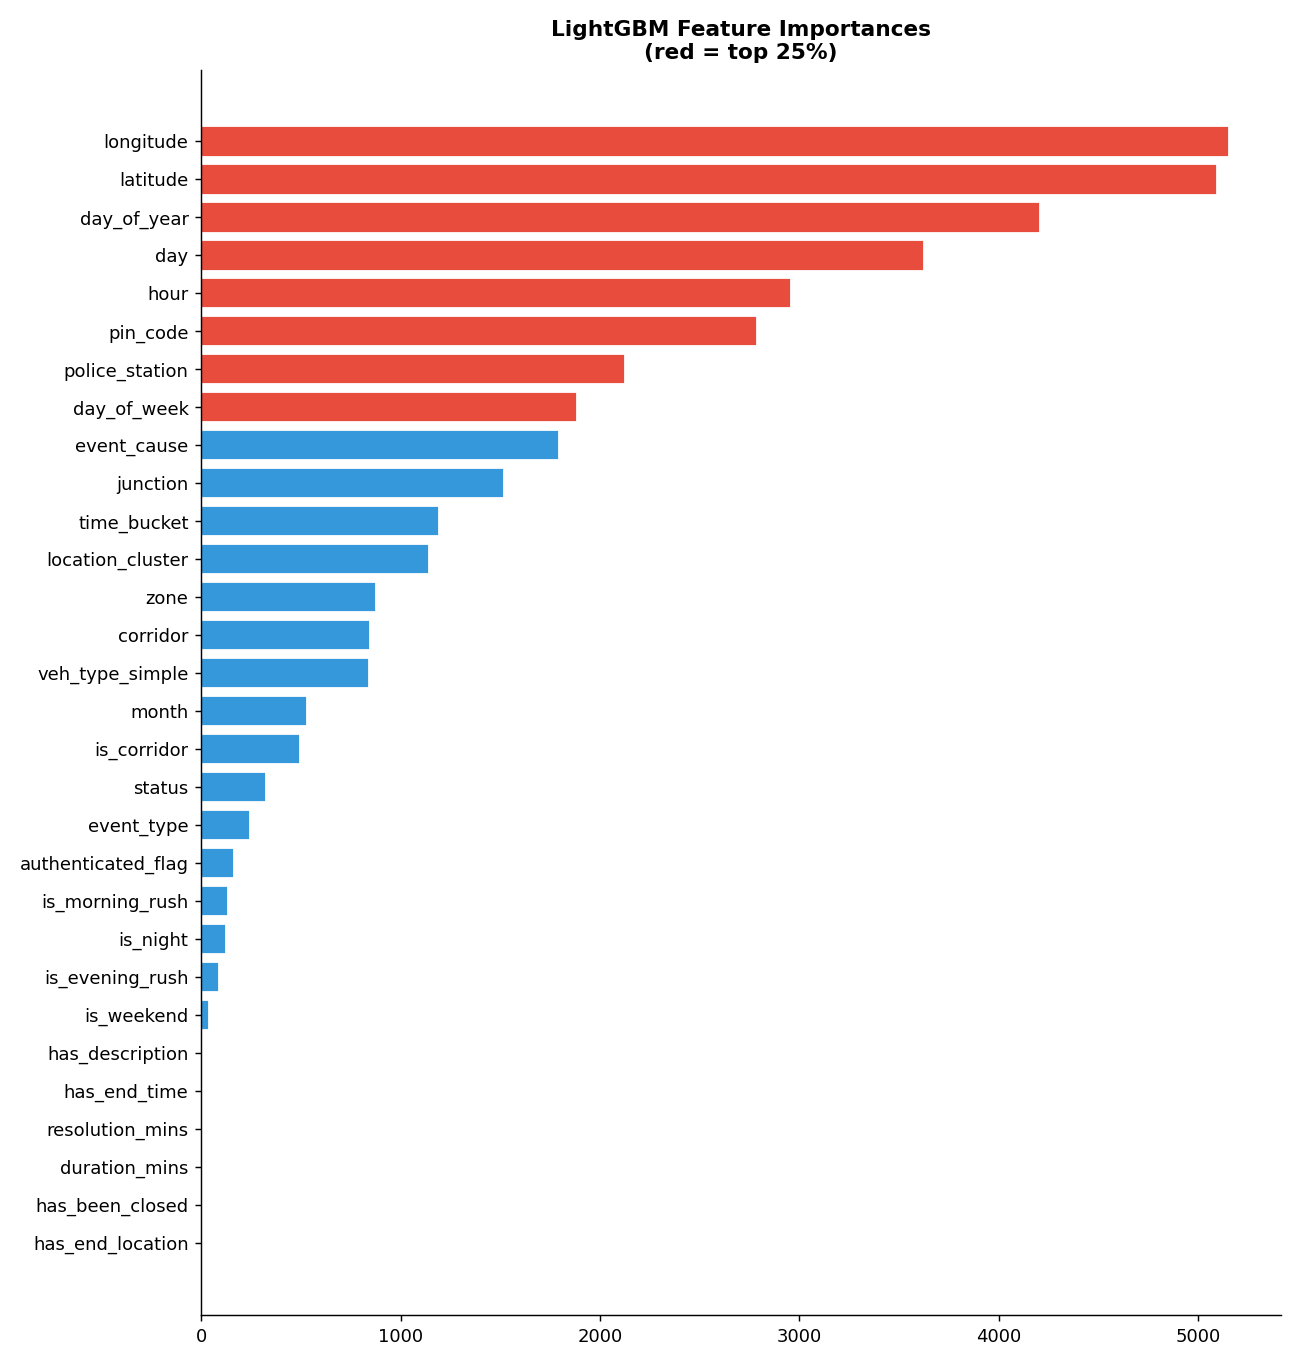
\includegraphics[width=0.7\textwidth]{chapters/7/figs/lgbm_feature_importance.png}
\caption{LightGBM feature importances (split count), red bars mark the top quartile.}
\label{fig:feature-importance}
\end{figure}

\section{Recommendation Engine: Demonstration}
\label{sec:recommendation-demo}

Table~\ref{tab:recommendation-demo} shows the rule-based recommendation engine's output for four representative scenarios, one at each severity level, illustrating how the base severity-to-action mapping in Table~\ref{tab:base-recommendation} is adjusted by corridor and peak-hour context.

\begin{table}[!h]
\centering
\caption{Recommendation engine output for four demonstration scenarios.}
\label{tab:recommendation-demo}
\small
\begin{tabular}{p{3.3cm}p{1.6cm}p{2.6cm}p{2.6cm}p{2.9cm}}
\toprule
Scenario & Manpower & Barricading & Diversion & Special action \\
\midrule
Low, vehicle breakdown, non-corridor, 14:00 & 2--4 officers & Cones only & None & -- \\
\addlinespace
Medium, water-logging, non-corridor, 09:00 (peak) & 5--10 officers & Partial barricade & Advisory route & Peak-hour +25\% flagged \\
\addlinespace
High, public event, corridor, 18:00 (peak), planned & 13--23 officers & Full barricade & Mandatory diversion & Crowd-control perimeter; pre-deploy $\geq$2h \\
\addlinespace
Critical, public event, corridor, 19:00 (peak), planned & 26--43 officers & Full corridor lockdown & Police-escorted diversion & Crowd-control perimeter; pre-deploy $\geq$2h \\
\bottomrule
\end{tabular}
\end{table}

The High- and Critical-severity ranges in Table~\ref{tab:recommendation-demo} (13--23 and 26--43 officers) are exactly what falls out of applying both the corridor multiplier ($\times 1.4$) and the peak-hour multiplier ($\times 1.25$) to the base ranges in Table~\ref{tab:base-recommendation}, which confirms the contextual-adjustment logic is behaving as designed rather than by coincidence.

\section{Summary of Findings}

Three conclusions fall out of the results above. First, every model tested is capable of predicting overall severity with high accuracy, which says the engineered feature set genuinely carries a strong signal -- this is not a case where the modelling choices are struggling against unusable inputs. Second, that shared high accuracy conceals a large, consistent gap in how well each model detects the minority classes, and the two class-weighted tree models (LightGBM and XGBoost) are noticeably more dependable on the operationally important Medium and Critical classes than either neural model trained without explicit class weighting here. Third, the rule-based recommendation layer, despite being intentionally simple and entirely deterministic, does successfully turn a bare severity label into a differentiated, context-sensitive operational plan, which supports the two-stage ``predict, then decide'' design chosen for this system back in Section~\ref{sec:recommendation-engine}.

\section{Limitations}

A few limitations are worth stating plainly. The severity label itself is a constructed proxy, built from two administrative fields rather than an independently annotated ground truth, so what the models are really learning to reproduce is this particular labelling policy -- not necessarily an external, universally agreed notion of ``true'' severity. The evaluation rests on a single stratified train/test split rather than repeated cross-validation, so the reported numbers carry some sampling variance, and that variance is largest precisely for the rare Medium and Critical classes where each percentage point corresponds to only a handful of events. Finally, the system has been tested only offline against historical records; it has not been run in a live control room, and its recommendations have not been checked against what a human operator would actually have decided for the same events.

\section{Conclusion and Future Scope}
\label{sec:future-scope}

This thesis set out to build, end to end, a system that predicts event-driven traffic-congestion severity and turns that prediction into an actionable resource recommendation, using a real, anonymised log of 8{,}173 Bengaluru traffic events. Four classifiers with different structural biases were trained and combined through a stacked ensemble, and every one of them was evaluated with explicit, front-loaded attention to class imbalance rather than accuracy alone. The headline result is that overall accuracy is a poor proxy for real usefulness here: only the class-weighted tree models, and to a lesser extent the stacked ensemble, achieve acceptable recall on the rare but safety-critical Critical class, which has direct implications for how a system like this would need to be tuned -- and which model would need to be chosen -- before any real deployment.

A few concrete directions follow naturally from what the results exposed.

\begin{itemize}
\item \textbf{Explicit class-imbalance handling.} Systematically compare class-weighting, SMOTE-based oversampling~\cite{chawla2002smote}, and decision-threshold adjustment specifically for the Medium and Critical classes, and measure their effect on macro-F1 and Critical recall rather than assuming any one of them is sufficient on its own.
\item \textbf{Ablation studies.} Isolate the individual contribution of the K-Means location-cluster feature and of the stacking step itself by comparing performance with and without each component, holding everything else fixed.
\item \textbf{Richer real-time context.} Bring in live weather data, a real-time traffic-flow feed, and road-network graph structure to complement the currently static, event-record-based feature set.
\item \textbf{Independent severity ground truth.} Where feasible, replace or augment the current priority/closure-derived label with severity judgements from an independent source -- for instance, retrospective control-room review -- to check whether the models are learning genuine severity signal or only the administrative labelling policy behind Table~\ref{tab:target-construction}.
\item \textbf{Field pilot.} Run the inference pipeline alongside real human traffic-control decision-making in a controlled pilot, comparing recommended and actual resource allocations, and use that comparison to refine the rule-based engine iteratively.
\end{itemize}
